\documentclass[utf8x, 12pt]{G7-32} 


% --------- -------- SETTINGS --------- --------

% --------- Настройки стиля ГОСТ 7-32 --------

% Гипертекстовое оглавление в PDF
\usepackage[
bookmarks=true, colorlinks=true, unicode=true,
urlcolor=black,linkcolor=black, anchorcolor=black,
citecolor=black, menucolor=black, filecolor=black,
]{hyperref}

\usepackage{graphicx}   % Пакет для включения рисунков
\DeclareGraphicsExtensions{.jpg,.pdf,.png}
\geometry{right=20mm}
\geometry{left=30mm}
\usepackage{enumerate}
\setcounter{tocdepth}{3} % Подробность оглавления


% --------- other settings --------
\usepackage{MnSymbol}
%\usepackage{simpsons}
% --------- -------- SETTINGS --------- --------



\begin{document}

\frontmatter 

% --------- -------- TITLE --------- --------

\begin{center} 

\large САНКТ-ПЕТЕРБУРГСИЙ ГОСУДАРСТВЕННЫЙ ПОЛИТЕХНИЧЕСКИЙ УНИВЕРСИТЕТ

\large Кафедра Компьютерных Систем и Программных Технологий \\[5.5cm] 

\huge ОТЧЕТ \\[0.6cm] % название работы, затем отступ 0,6см
\large по лабораторной работе №3\\
\large Тема: <<Программа для шифрования и подписи GPG, пакет Gpg4win>>\\
\large Дисциплина: <<Методы и средства защиты информации>>\\[3.7cm]

\end{center} 

\begin{flushright}
Выполнил: студент гр. 53501/2 \\
Федоров Е.М. \\[1.2cm]


Преподаватель \\
Вылегжанина К.Д.
\end{flushright}


\vfill 

\begin{center} 
\large Санкт-Петербург \\
2015
\end{center} 

\thispagestyle{empty}


% --------- -------- TITLE --------- --------

\thispagestyle{empty}
\setcounter{page}{0}
\tableofcontents
\clearpage
\mainmatter


\chapter{Задание}

\begin{enumerate}
	\item Изучить документацию,запустить графическую оболочку Kleopatra
	\item Создать ключевую пару OpenPGP (File $\rightarrow$ New Certificate)
	\item Экспортировать сертификат (File $\rightarrow$ Export Certificate)
	\item Поставить ЭЦП на файл (File $\rightarrow$ Sign/Encrypt Files)
	\item Получить чужой сертификат из репозитория, файл с данными и файл с сигнатурой
	\item Импортировать сертификат, подписать его
	\item Проверить подпись
	\item Взять сертификат кого-либо из коллег, зашифровать и подписать для него какой--либо текст, предоставить свой сертификат, убедиться, что ему удалось получить открытый текст, проверить подпись
	\item Предыдущий пункт наоборот
	\item Используя GNU Privacy handbook (ссылка в материалах) потренироваться в использовании gpg через интерфейс командной строки, без использования графических оболочек.
\end{enumerate}


\chapter{Выполнение}

\section{Создать ключевую пару OpenPGP (File $\rightarrow$ New Certificate)}

\begin{figure}[hhh!]
	\begin{center}
		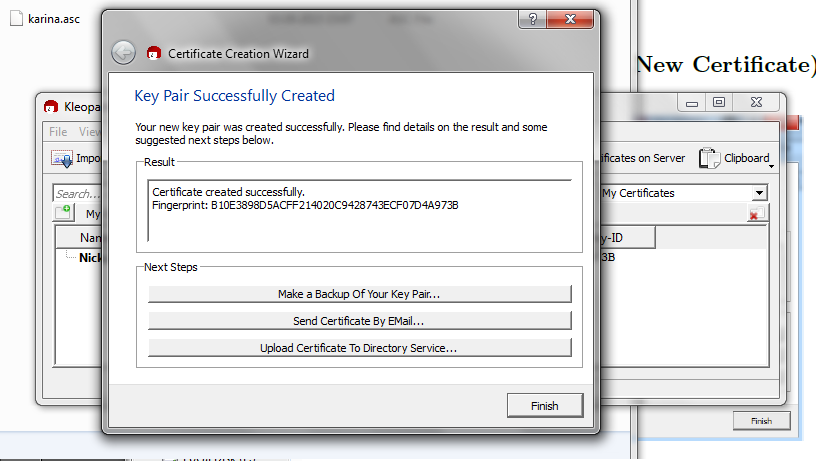
\includegraphics[width=10cm]{img2/21}
		
	\end{center}
\end{figure}	



\newpage

\section{Поставить ЭЦП на файл (File $\rightarrow$ Sign/Encrypt Files)}

Создадим файл <<test.txt>>, чтобы впоследствии зашифровать его.

\begin{figure}[hhh!]
	\begin{center}
		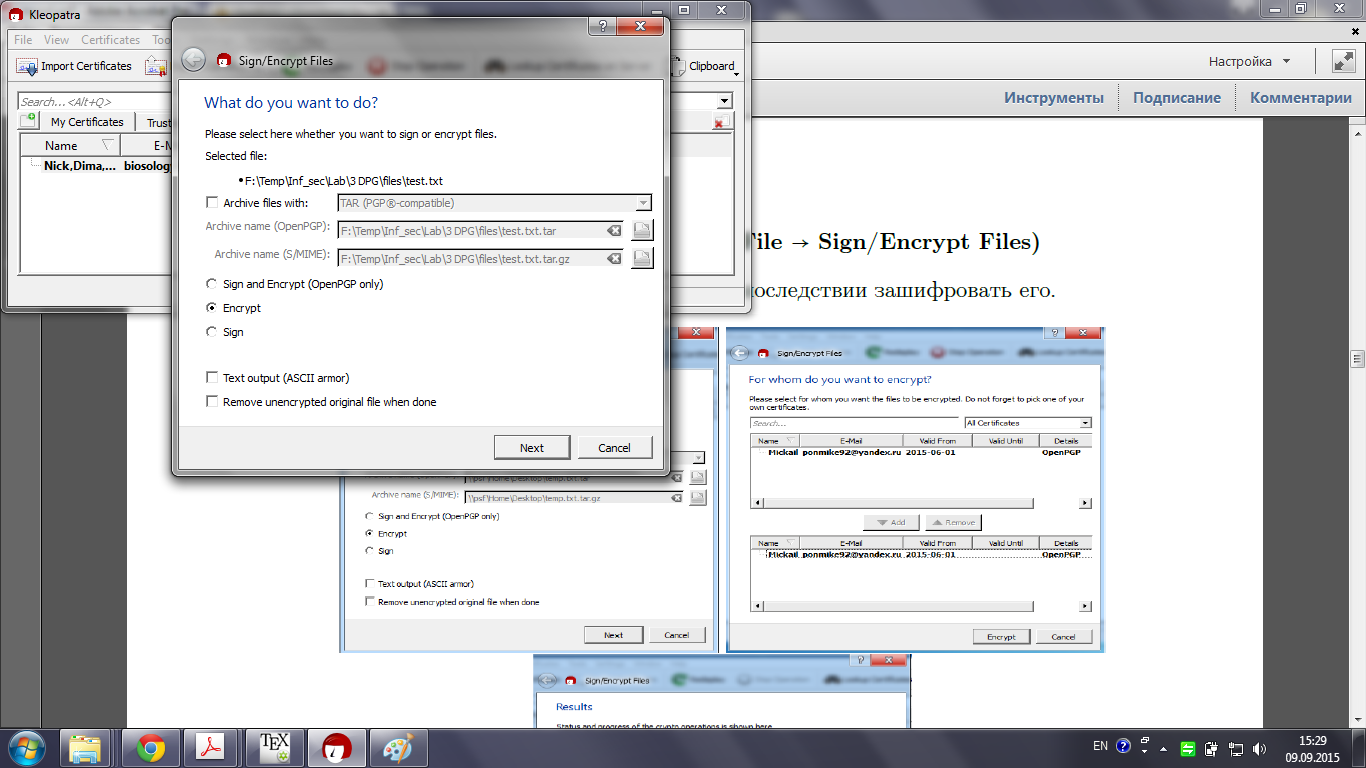
\includegraphics[height=6cm]{img2/231}
		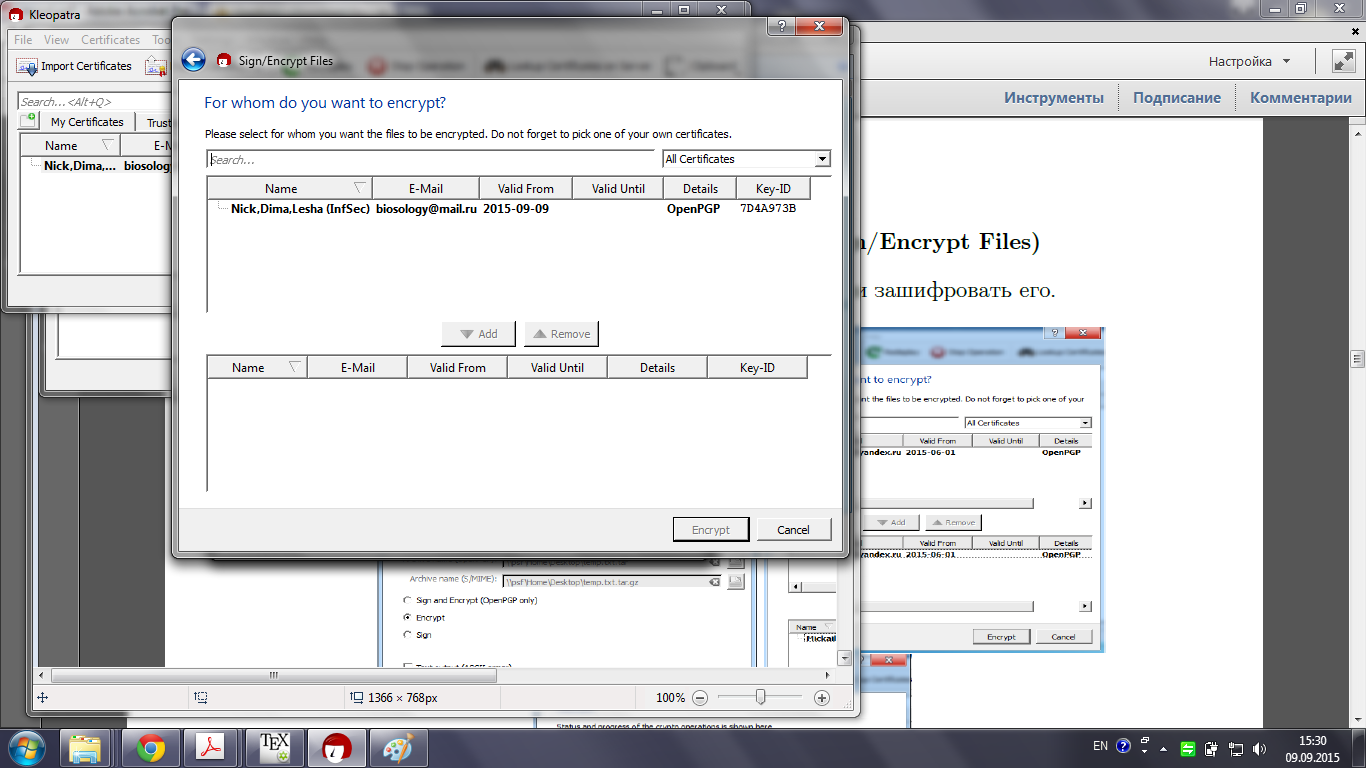
\includegraphics[ height=6cm]{img2/232}
		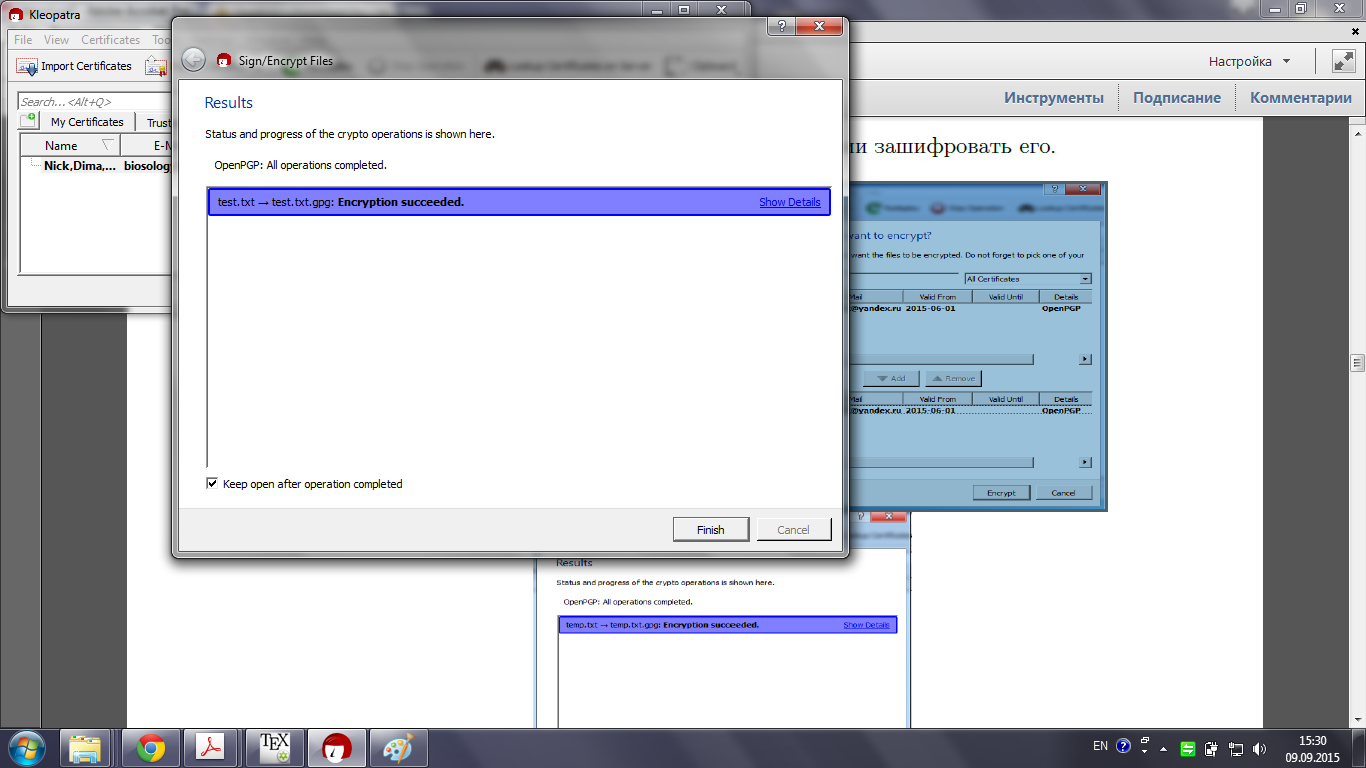
\includegraphics[height=6cm]{img2/233}
	\end{center}
\end{figure}	

В ходе шифрования нас попросят ввести фразу--пароль. 


\section{Получить чужой сертификат из репозитория, файл с данными и файл с сигнатурой}

	

\newpage

\section{Импортировать сертификат, подписать его}

Импортируем сертификат:
\begin{figure}[hhh!]
	\begin{center}
		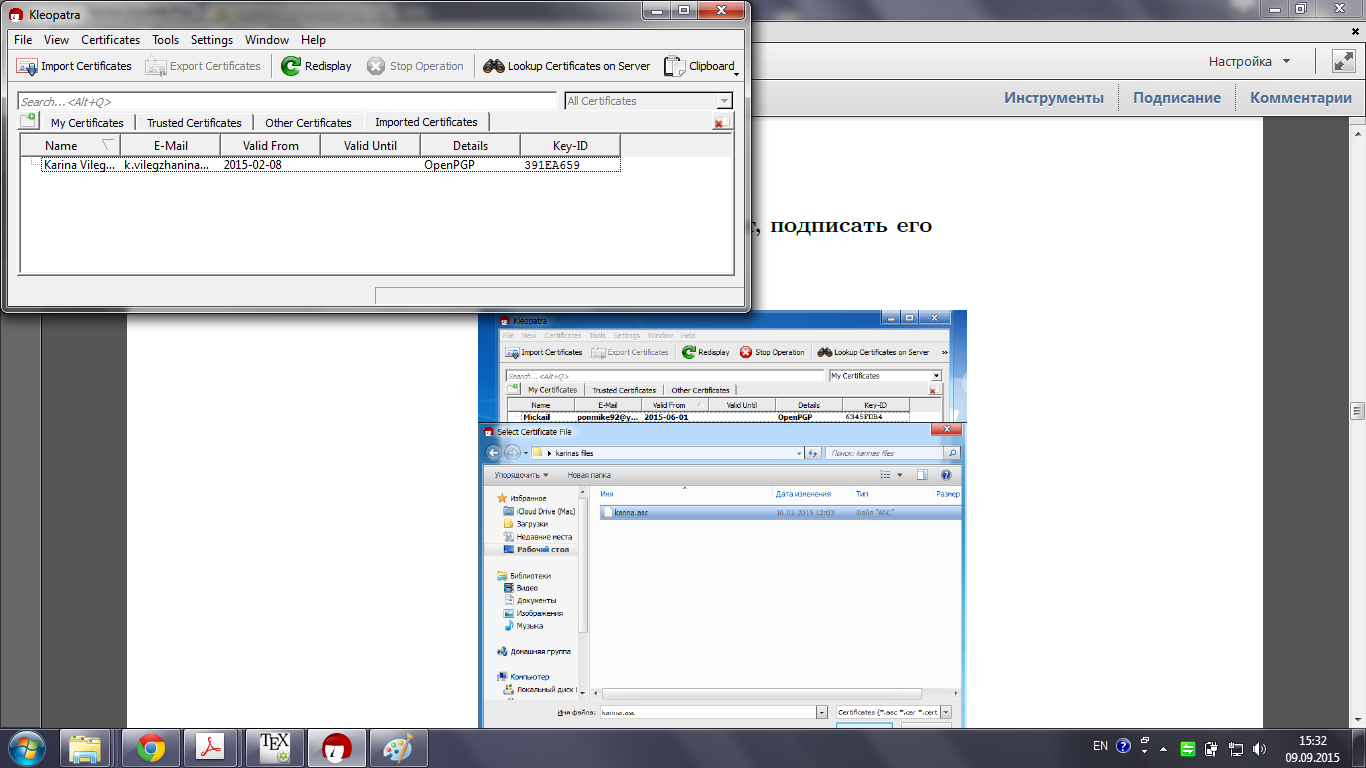
\includegraphics[width=9cm]{img2/25}
	\end{center}
\end{figure}	


Подпишем сертификат:
\begin{figure}[hhh!]
	\begin{center}
		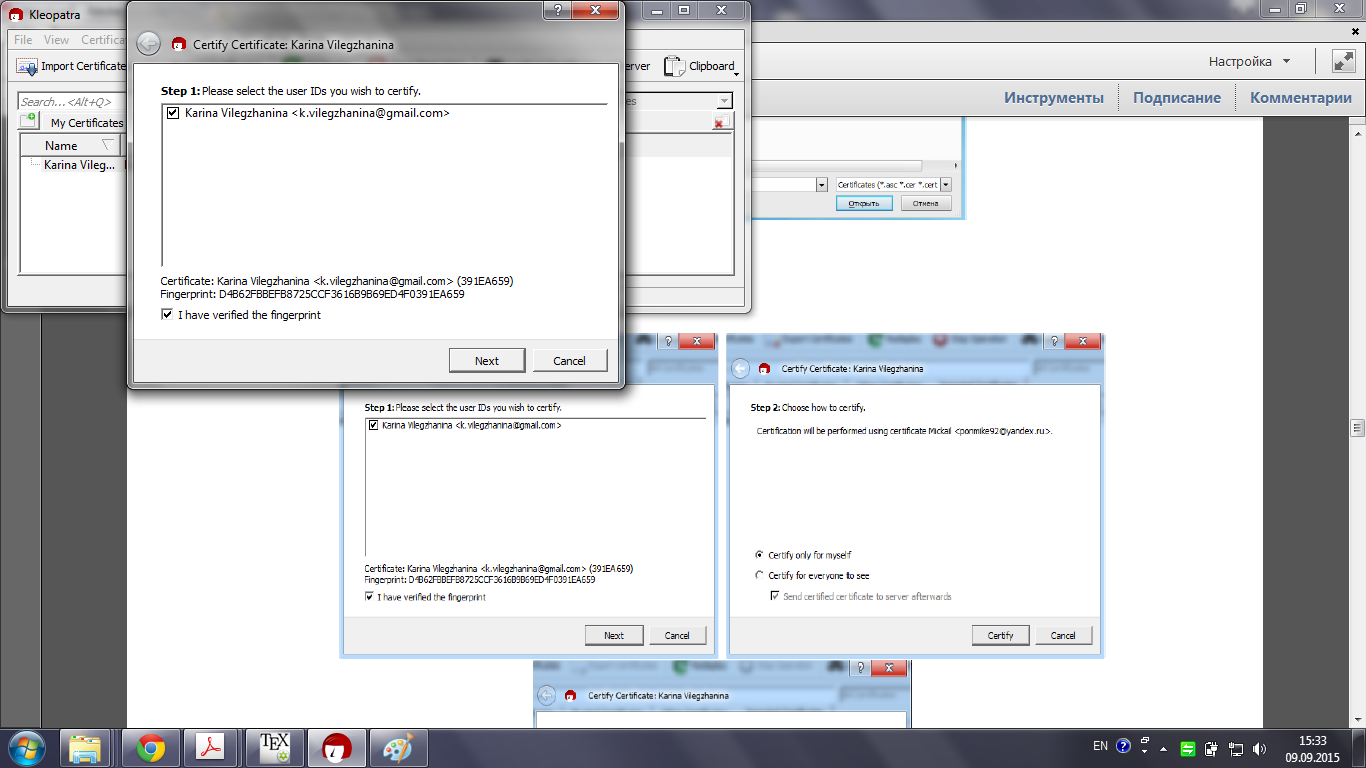
\includegraphics[width=7cm, height=6cm]{img2/252}
		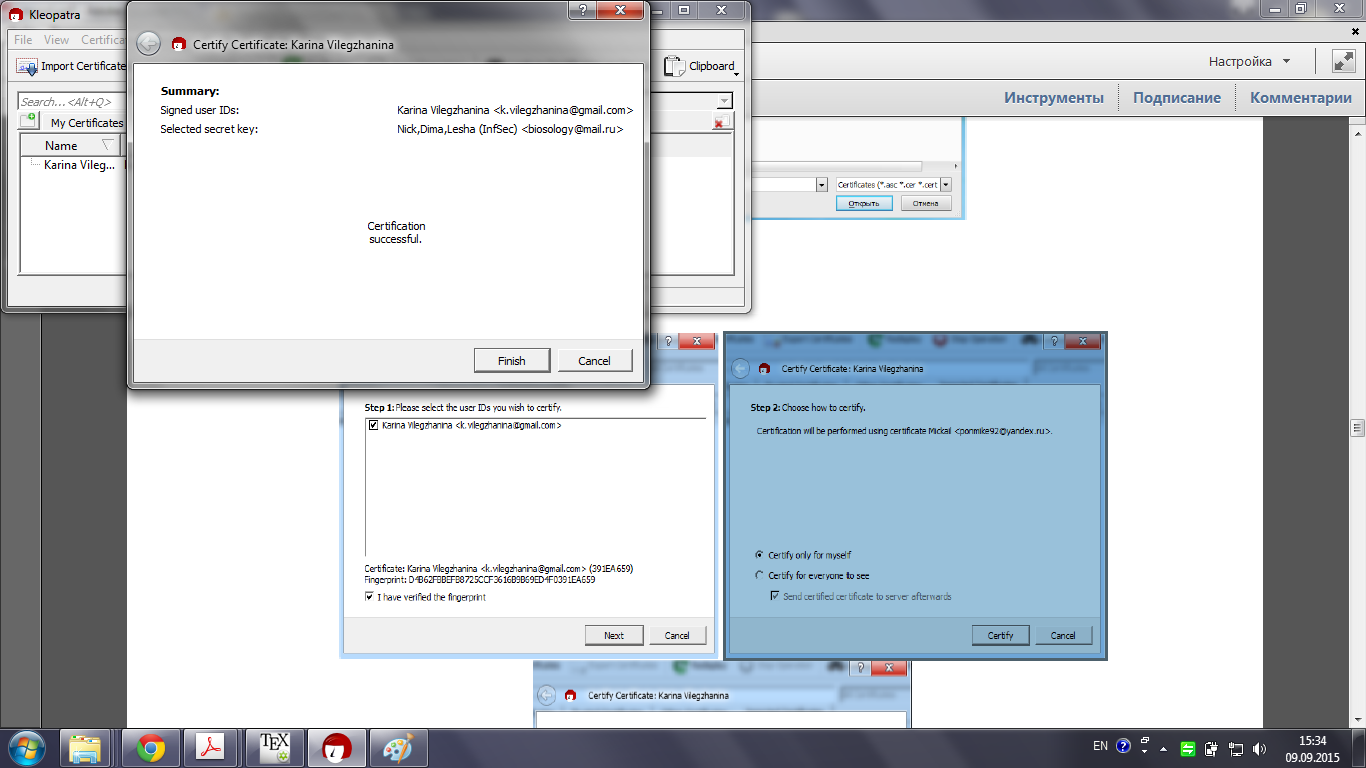
\includegraphics[width=7cm, height=6cm]{img2/253}
		
	\end{center}
\end{figure}	


 \newpage
\section{Проверить подпись}
\begin{figure}[hhh!]
	\begin{center}
		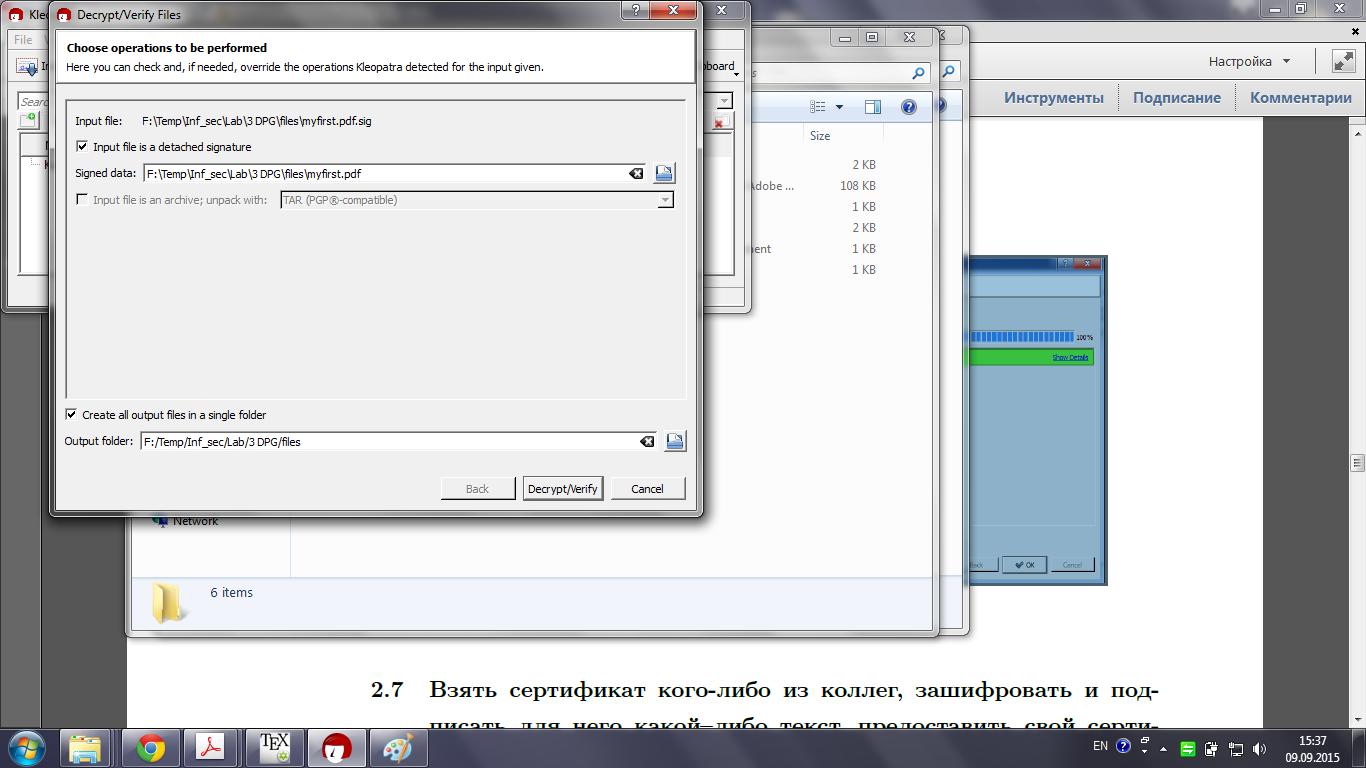
\includegraphics[width=7cm, height=6cm]{img2/261}
		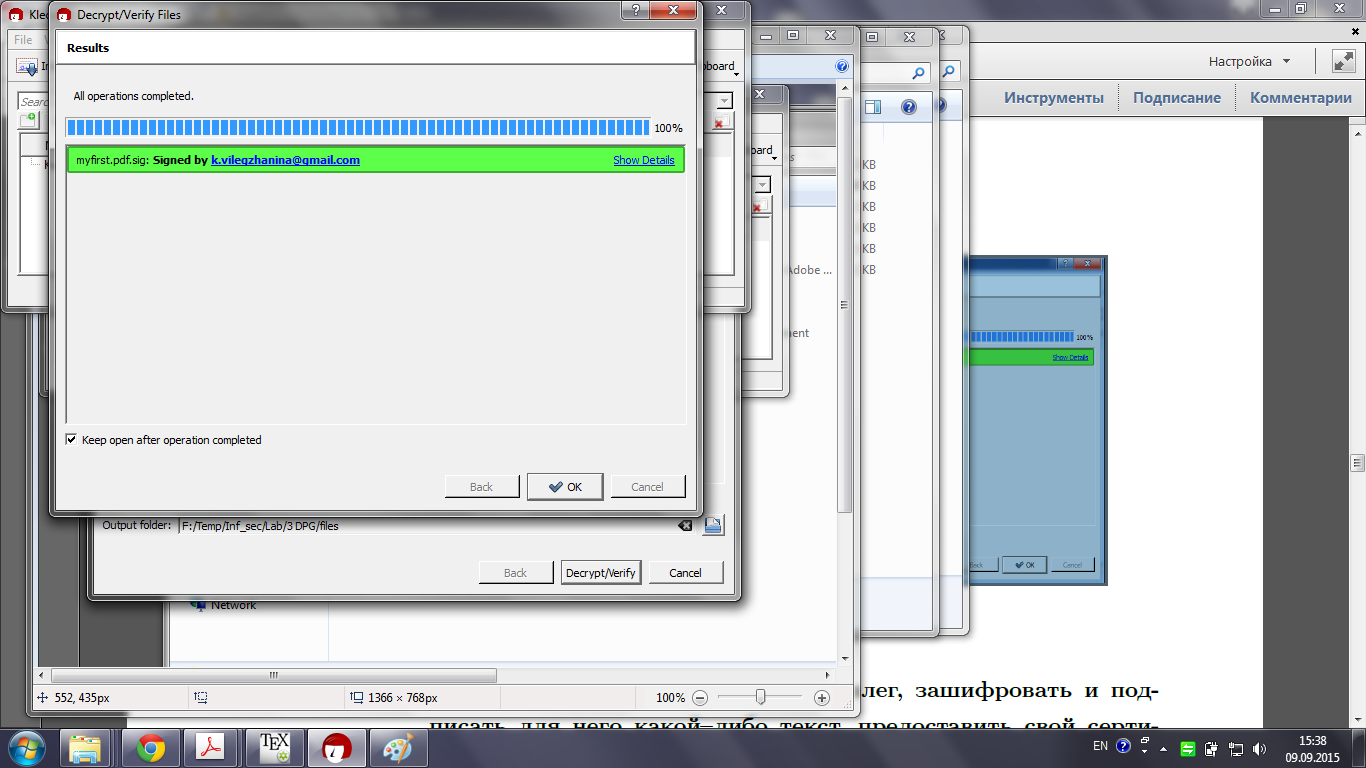
\includegraphics[width=7cm, height=6cm]{img2/262}
	\end{center}
\end{figure}	


\section{Взять сертификат кого-либо из коллег, зашифровать и подписать для него какой--либо текст, предоставить свой сертификат, убедиться, что ему удалось получить открытый текст, проверить подпись}

Сертификат был взят преподавательский. Для дальнейшего шифрования был использован файл <<test.txt>>.

\begin{figure}[hhh!]
	\begin{center}
		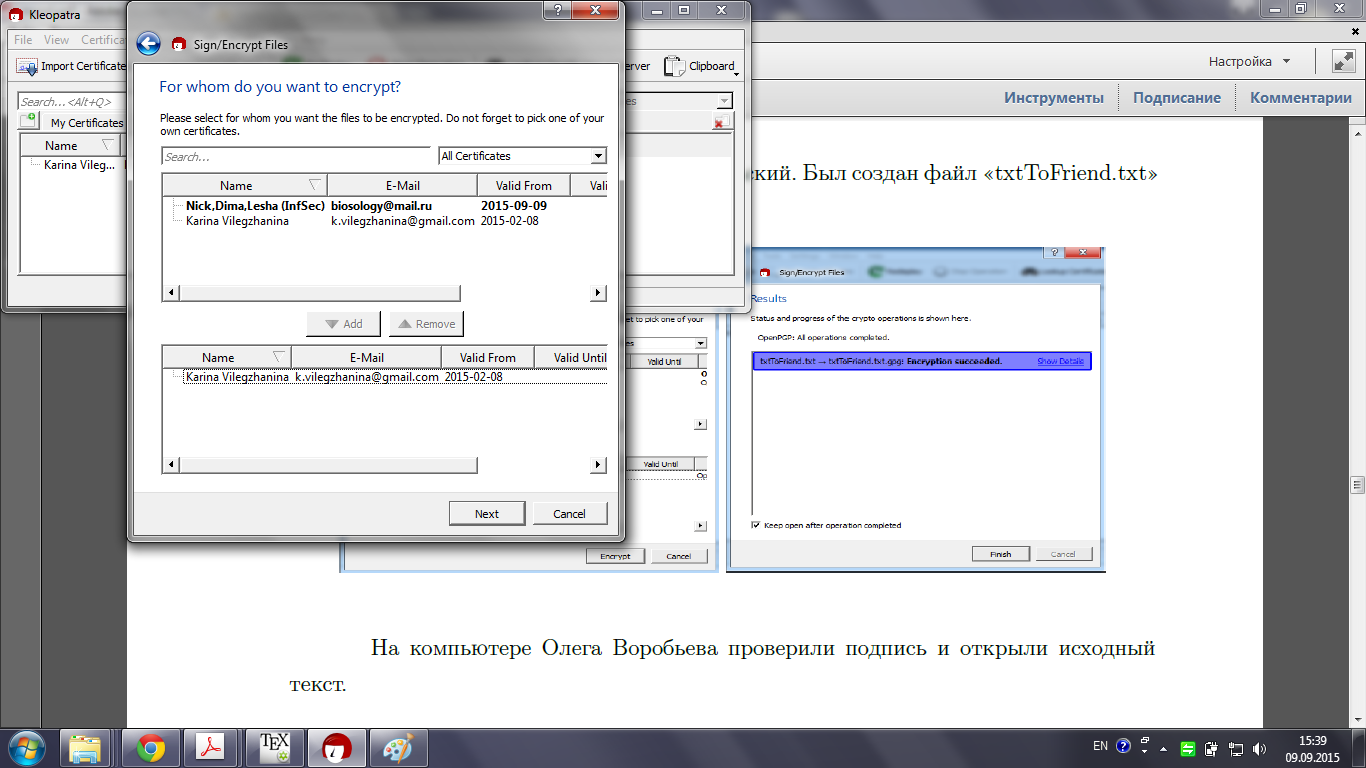
\includegraphics[height=6cm]{img2/271}
		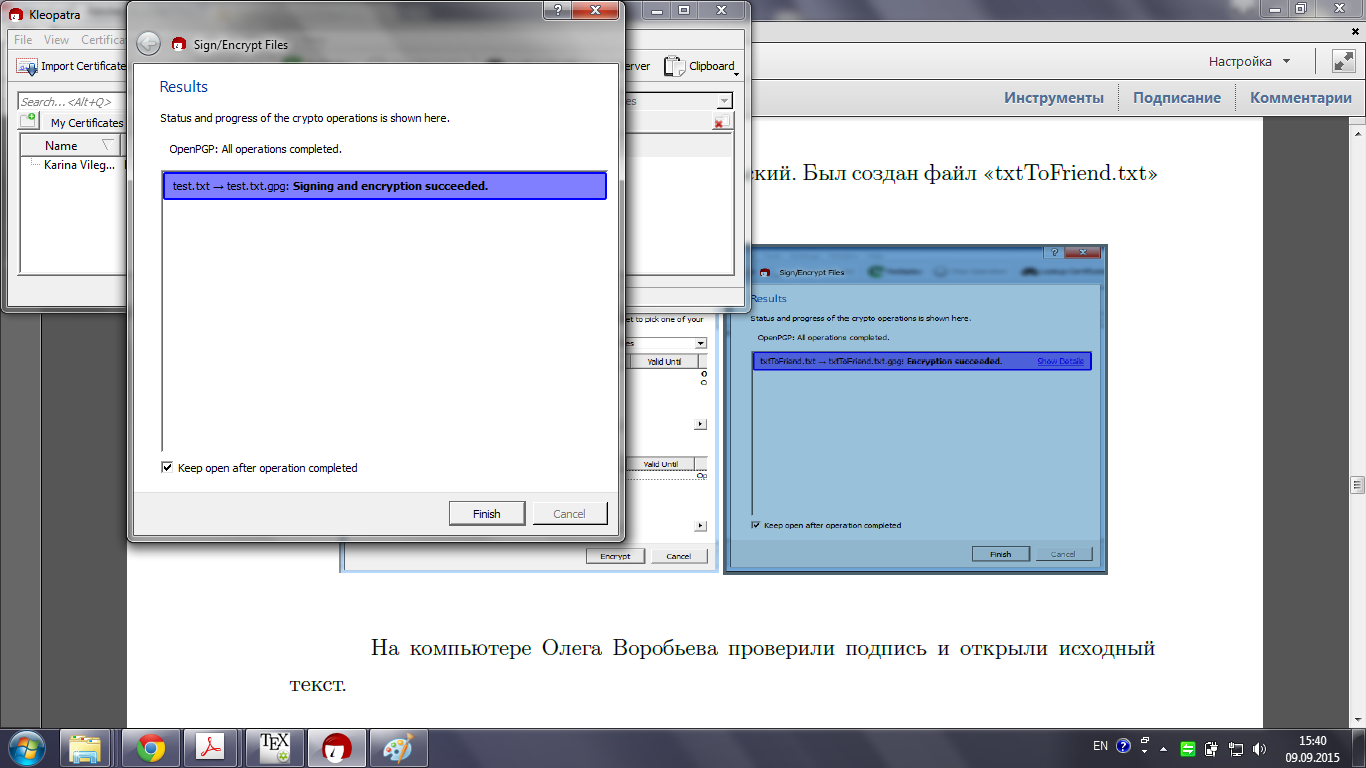
\includegraphics[height=6cm]{img2/272}
	\end{center}
\end{figure}	

На другом компьютере проверили подпись и открыли исходный текст.

\newpage

\section{Используя GNU Privacy handbook (ссылка в материалах) потренироваться в использовании gpg через интерфейс командной строки, без использования графических оболочек.}

Были изучены следующие команды:

\begin{itemize}
	\item –gen-key --- создание новой пары ключей
	\item –sign --- создает подпись для указанных файлов
	\item –encrypt --- указывает на то, что данные надо зашифровать
	\item –symmetric --- используется для шифрования файла
	\item –decrypt --- расшифровывает указанные файлы и сохраняет результат
	\item –verify --- проверяет подписи для указанных файлов
	\item –list-keys --- выводит список всех открытых ключей
	\item –delete-key --- удаляет открытый ключ из списка. 
	\item –export (–import) --- экспорт/импорт ключей
\end{itemize}

\medskip

Создадим пару GPG ключей, для этого наберём команду в терминале <<gpg --gen-key>> в той папке, в которой мы хотим создать ключ.

\begin{figure}[hhh!]
	\begin{center}
		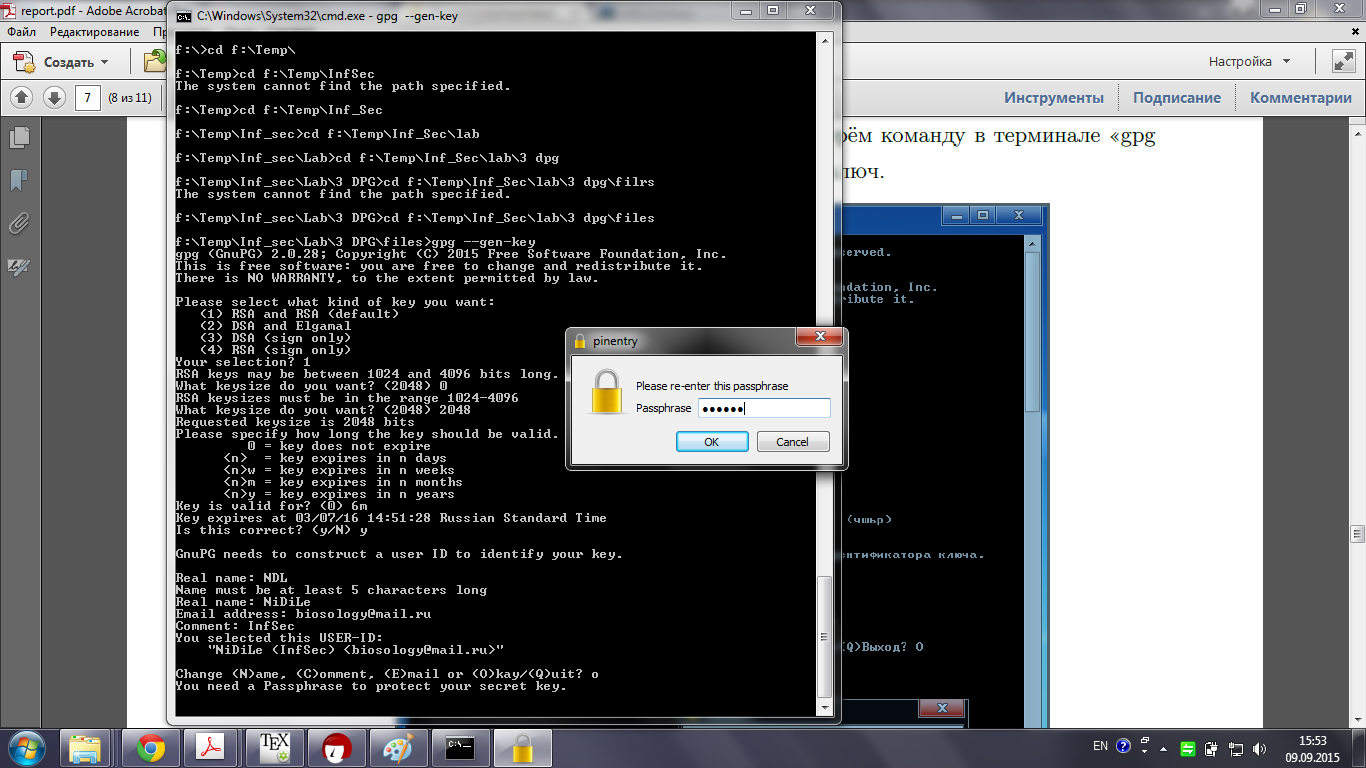
\includegraphics[width=12cm]{img2/281}
	\end{center}
\end{figure}	


Выведем список доступных ключей, для этого наберём команду \linebreak <<gpg --list-keys>>

\begin{figure}[hhh!]
	\begin{center}
		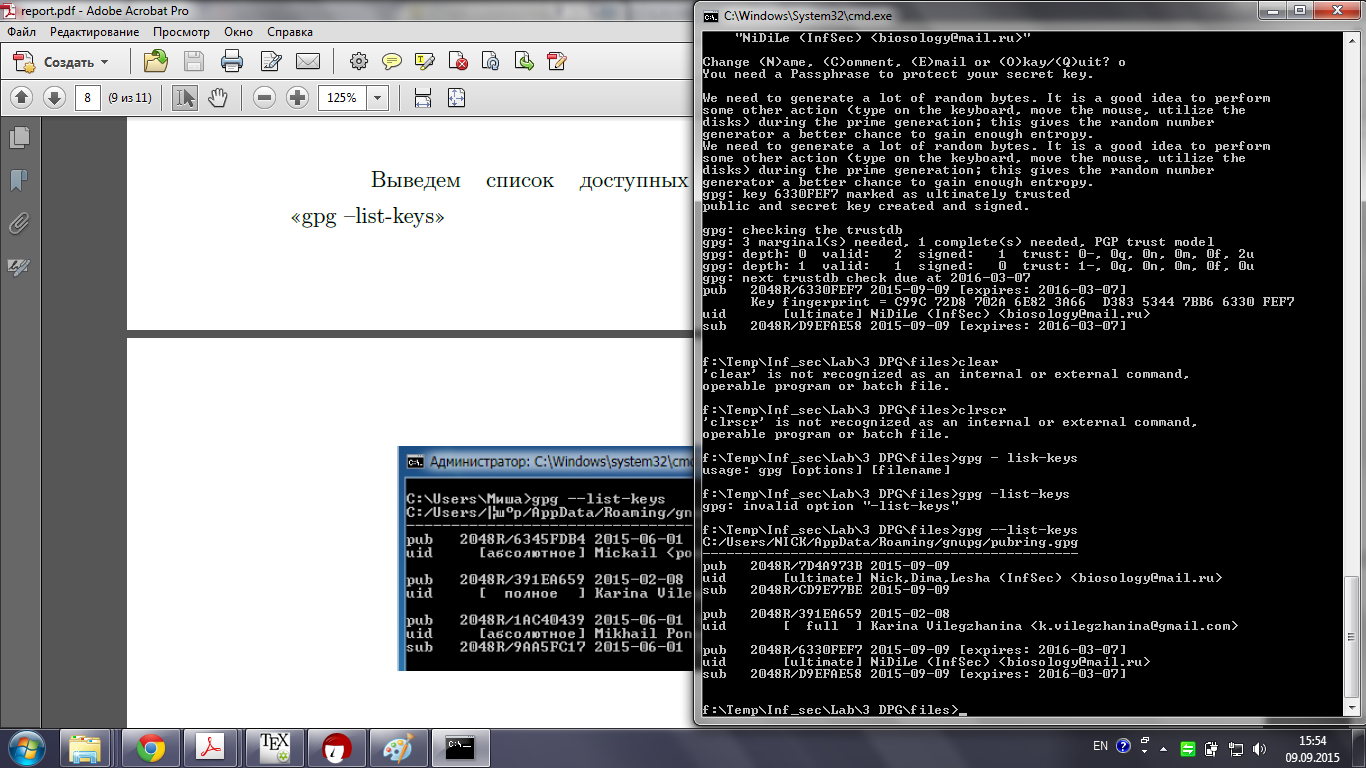
\includegraphics[width=12cm]{img2/282}
	\end{center}
\end{figure}	

Экспортируем ключ

\begin{figure}[hhh!]
	\begin{center}
		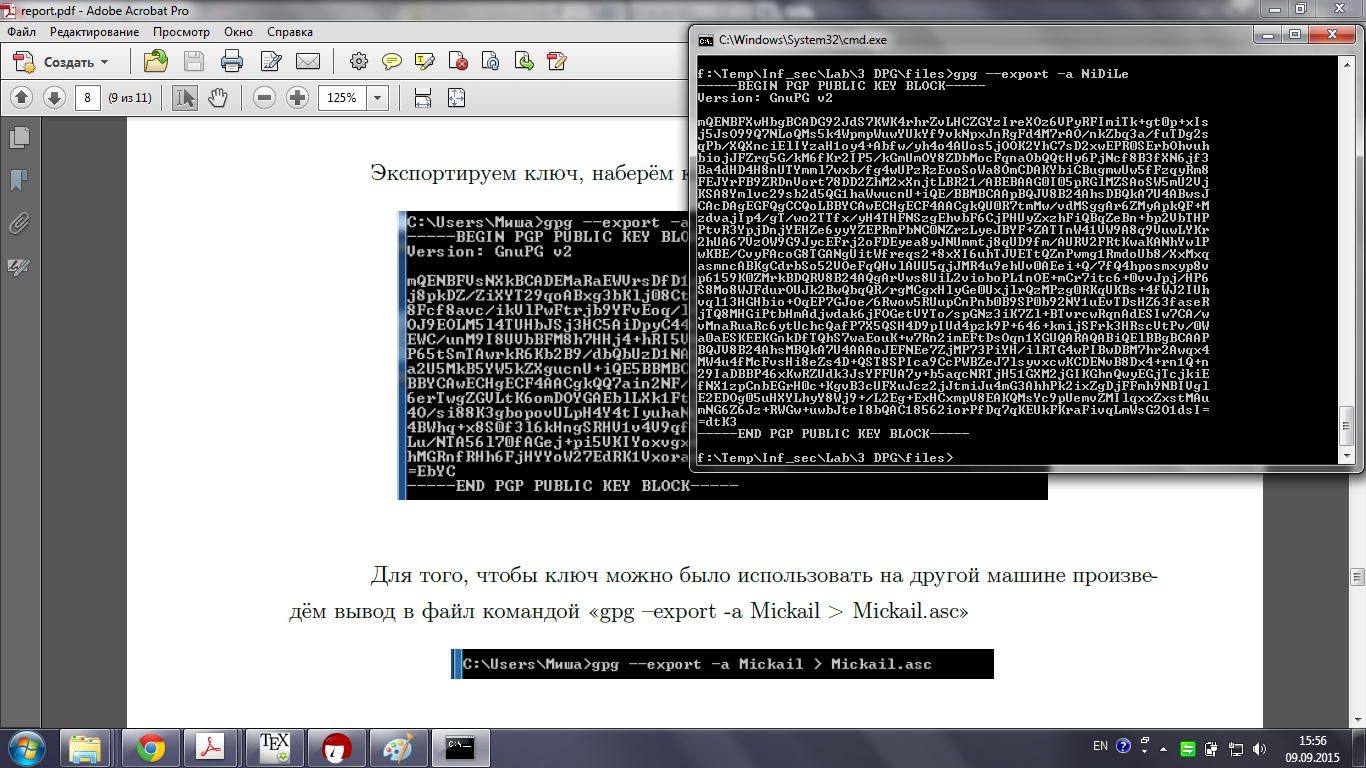
\includegraphics[width=12cm]{img2/283}
	\end{center}
\end{figure}	


Для того, чтобы ключ можно было использовать на другой машине произведём вывод в файл 

\begin{figure}[hhh!]
	\begin{center}
		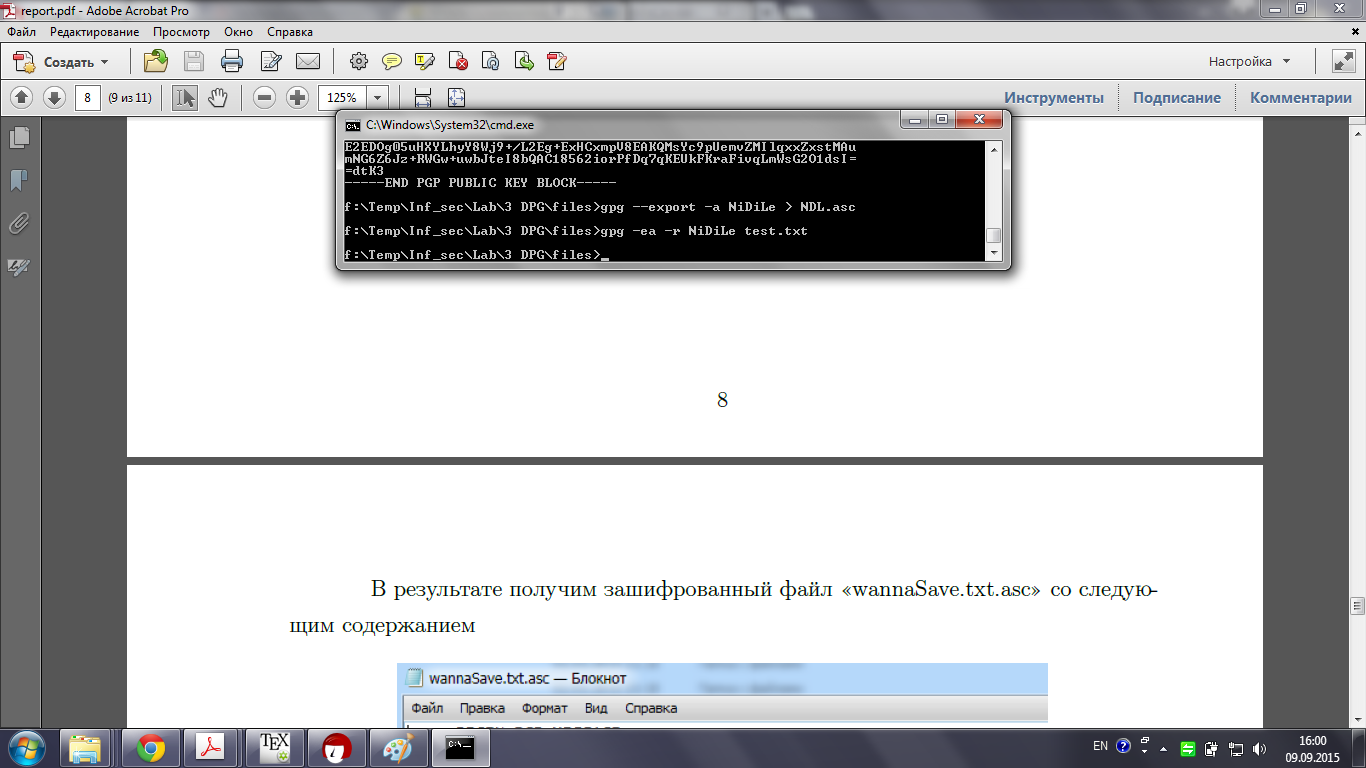
\includegraphics[width=10cm]{img2/284}
	\end{center}
\end{figure}	




\chapter{Выводы}

В ходе выполнения лабораторной работы была изучена программа Kleopatra, используемая для шифрования и подписи GPG. Познакомился с возможностями шифрования с помощью терминала. Появилось представление об электронной подписи файла, ключа и шифрования в целом.


\end{document}
